\begin{figure}
\centering
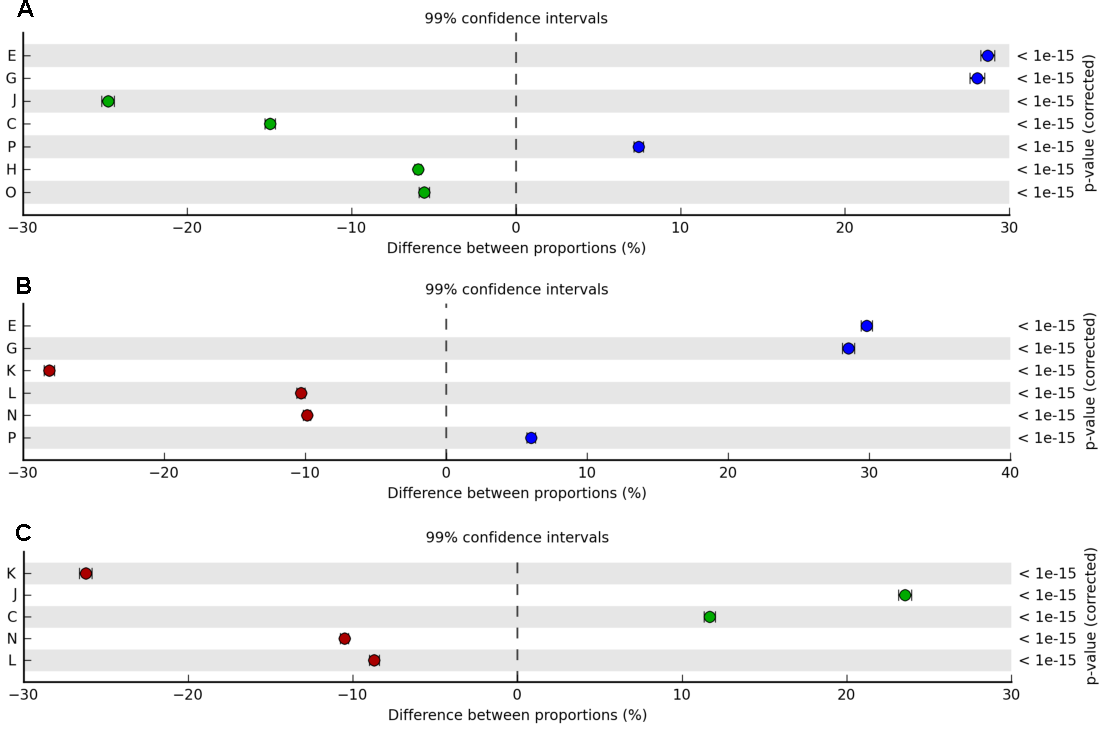
\includegraphics[width=\textwidth]{ace_figures/stamp.pdf}
\caption[Statistical analysis of Ace Lake metaproteome]{ Statistical analysis of normalised mass spectra from \ac{COG} annotated protein between each zone in Ace Lake. 
Proteins are shown grouped into \ac{COG} categories.
Only categories with corrected p-values $<$0.05 and effect size $>$5 are displayed.
(\textbf{A}) Mixolimnion compared to interface. 
(\textbf{B}) Mixolimnion compared to monimolimnion.
(\textbf{C}) Interface compared to monimolimnion. 
Blue, mixolimnion; green, interface; red, monimolimnion.
\ac{COG} category descriptions are: E, amino acid transport and metabolism; G, carbohydrate transport and metabolism; J, translation, ribosomal structure and biogenesis; C, energy production and conservation; P, inorganic ion transport and metabolism; H, co-enzyme transport and metabolism; O, post-translational modification, protein turnover and chaperones; K, transcription; L, replication, recombination and repair; N, cell motility.
}
\label{fig:stamp}

\end{figure}
